\documentclass[journal]{IEEEtran}

\usepackage{cite}
\usepackage{amsmath,amssymb,amsfonts,amsthm}
\theoremstyle{definition}
\newtheorem{criterion}{Criterion}
\usepackage{graphicx}
\graphicspath{{figures/}}
\usepackage{textcomp,xcolor,booktabs,array,url,enumitem,multirow}
\setlist{topsep=2pt,itemsep=1pt,parsep=0pt,leftmargin=*}
\usepackage{tikz}
\usetikzlibrary{positioning,arrows.meta,fit,backgrounds,automata,shapes.geometric,calc}
\usepackage{pgfplots}
\pgfplotsset{compat=1.18,table/col sep=comma}
\usepgfplotslibrary{groupplots}
\emergencystretch=1em
\renewcommand{\topfraction}{0.92}
\renewcommand{\bottomfraction}{0.75}
\renewcommand{\textfraction}{0.07}
\renewcommand{\floatpagefraction}{0.88}
\setcounter{topnumber}{3}
\setcounter{bottomnumber}{2}
\setcounter{totalnumber}{4}
\setlength{\textfloatsep}{6pt plus 2pt minus 2pt}
\setlength{\floatsep}{4pt plus 2pt minus 2pt}
\setlength{\dblfloatsep}{6pt plus 2pt minus 2pt}
\setlength{\dbltextfloatsep}{6pt plus 2pt minus 2pt}
\setlength{\intextsep}{4pt plus 2pt minus 2pt}
\setlength{\abovecaptionskip}{3pt}
\setlength{\belowcaptionskip}{0pt}
\usepackage[normalem]{ulem}   % normalem mantiene \emph in corsivo
\usepackage{xcolor}

\newcommand{\del}[1]{{\color{blue}\sout{#1}}}  % testo rimosso: blu barrato
\newcommand{\add}[1]{{\color{red}#1}}          % testo aggiunto: rosso
\newcommand{\nongiust}[1]{{\color{red}[NON GIUSTIFICATO NEGLI ALLEGATI: #1]}}
\newcommand{\todoM}{{\color{red}[TODO: risultato M6/M7]}}

\begin{document}

\title{DIB: Managing Local MUD Policy Lifecycles with Shared IoT Traffic Evidence}
\author{Anonymous Authors}
\maketitle

\begin{abstract}
Shared IoT traffic observations can help administrators create Manufacturer Usage Description (MUD) policies when manufacturer profiles are unavailable or outdated.
In the event of compromise, their lifecycle may require coordinated withdrawal while preserving local control over permissions.

This paper presents Device Intent Blueprint (DIB), a framework designed to facilitate the creation and sharing of MUD policies by separating shared traffic evidence from local authorization. Candidate communications enter a review queue and generate MUD rules only after local approval.  A shared dispute triggers coordinated withdrawal while local decisions are preserved. DIB records the approval validity and the origin of revocation, allowing disconnected sites to reconcile even after missing an entire withdrawal-and-restoration episode.

 We evaluate DIB through bounded (finite-instance) exhaustive lifecycle model checking, an OpenWrt/osMUD testbed, and experiments on three IoT traffic datasets. The results show that DIB works as intended: it preserves local authorization during coordinated withdrawal and recovery, reconciles a restarted site with median convergence within a pre-registered bound, and supports flexible candidate selection. A protocol-level model exposed races between evidence reads and local updates, one of which lets an approval survive a restoration; the corrected design is verified in the model and implemented in the evaluated prototype. 
\end{abstract}

\begin{IEEEkeywords}
IoT security, Manufacturer Usage Description, distributed network management, access policy management, policy lifecycle.
\end{IEEEkeywords}

\section{Introduction}
\label{sec:introduction}
Internet of Things (IoT) devices rely on network services for updates, remote control, and data exchange. Restricting their communications to the services they need can limit their exposure and the network activity of compromised devices~\cite{mirai,hernandezramos2021mudreview}. To support this approach, the Internet Engineering Task Force (IETF) standardized Manufacturer Usage Description (MUD) in RFC~8520~\cite{rfc8520}. This standard involves MUD files, describing a device's intended communications, and MUD managers, which translate this description into access-control rules for the local networks.

Since manufacturer profiles may be unavailable or become outdated as firmware and cloud services change~\cite{hernandezramos2021mudreview,allowlistvariability}, traffic observations can help administrators draft or update these profiles, and reports from other networks provide additional evidence when local observations remain limited. However, a service used in one network may be unnecessary in another, and observed traffic may include communications generated by compromised devices~\cite{allowlistvariability,mirai}. Therefore, administrators must decide which proposed rules to apply in their own networks.

These decisions are part of a policy lifecycle. For instance, considering a camera without a manufacturer profile: two networks observe the same cloud service, and an administrator uses their reports to approve a local rule. If a contributor later disputes that service, the participating networks must withdraw the associated permissions. Once the dispute is resolved, the system must distinguish dispute-induced withdrawal from independent local revocation. It must preserve this distinction when reconciling a network that was disconnected throughout the episode.

To overcome this limitation, this paper proposes \emph{Device Intent Blueprint (DIB)}, a framework for managing locally authorized MUD policies based on shared IoT traffic observations. We call each independently administered network a \emph{site}. DIB groups observations into \emph{endpoint facts}, each of which identifies a (i) device type, (ii) communication direction, (iii) protocol, (iv) peer, and (v) port. The observations and contributor reports supporting a fact form its \emph{evidence}, and a \emph{registry} stores that evidence alongside separate records of each site's policy decisions.

DIB separates candidate selection from authorization. Selected facts enter the MonitorOnly state, where administrators can review them without creating MUD rules.
Once an administrator approves locally, a fact is moved to the active state, and it can be exported to other sites. A shared dispute invalidates approvals; restoration requires renewed review and preserves local revocations. Ordered updates reconcile sites that missed intermediate changes.

Existing approaches cover profile extraction, evidence sharing, and coordinated authorization. DIB addresses recovery across independent authorities by combining deny-overrides and a last-writer-wins pending register with explicit approval validity and revocation origin. Together, these records determine whether a recovering site must return a fact to review or retain an independent local veto.

To conclude, the main contributions of this paper are:
(1)~a policy lifecycle and reconciliation mechanism that preserves local authorization during shared withdrawal and recovery, including after missed episodes;
(2)~a registry and distributed prototype, evaluated through finite-state verification, controlled ablations, recovery experiments, and OpenWrt/osMUD enforcement;
(3)~a matched evaluation on three IoT traffic datasets that distinguishes the effects of candidate admission and review ordering.


\section{Related Work}
\label{sec:related-work}

RFC~8520 leaves the local application of MUD recommendations to the network administrator and calls for policy updates to respect deployment-specific approval flows~\cite[Secs.~1.1 and~1.8]{rfc8520}. A parallel IETF effort standardizes MUD URL reissuance~\cite{mudacceptableurls}, which addresses authority over manufacturer URL updates. DIB governs operator-approved facts derived from traffic observations. Prior work extracts or enforces profiles from local traffic within one administrative domain~\cite{clearasmud, hamzatdsc, mudflow, CornoMannella2023GatewayMUD, osmud, mudscope} rather than governing observations shared across domains.

Threat-intelligence sharing platforms (MISP, STIX), contributor reputation systems~\cite{wagner2016misp, stix21, eigentrust, trustsurvey}, and collaborative IoT learning (CoLearn, D\"IoT, IoT Inspector)~\cite{colearn,ndiot2019, iotinspector, vasilomanolakis2015collaborative} aggregate evidence, traffic models, or anomaly reports. These approaches share information rather than grant network access, and therefore specify no withdrawal semantics for permissions already installed at a recipient.

Policy-based management and intent frameworks address policy specification, conflicts, and configuration~\cite{pbnm,rfc9315,alshaer2004firewall,chowdhary2022intent,pipeconf2022,vergutz2023data}. POLARIS~\cite{polaris} lets resource owners decide access from verifiable attributes and binds access to sessions. FIDEM~\cite{fidem} verifies device--MUD-class binding and propagates profile updates through URL reissuance or signature-change checks. Their workflows address identity-based access and profile authenticity, respectively. DIB assumes established identities and specifies how shared withdrawal invalidates per-site approvals, how restoration preserves local vetoes, and how sites reconcile after missed episodes. Dynamic and security-tested MUD profiles~\cite{blockchainmud,matheu2019mudtesting} also motivate profile evolution.

The deny-overrides combining rule in XACML and policy frameworks~\cite{xacml3} resolves conflicting decisions during policy evaluation. DIB retains the origin of a revocation across updates so that a shared restore preserves a local denial. Zanzibar~\cite{zanzibar} addresses stale authorization through consistency tokens in a globally coordinated service, where one authority both grants and revokes. DIB propagates withdrawal to sites that grant permissions independently and reconciles unreachable sites after reconnection. Its pending target follows a last-writer-wins register~\cite{crdt}, with local guards preserving revocation origin.

\textcolor{red}{Paragrafo qui in cui enfatizzi in cosa DIB è diverso/migliore e cosa pensi possa portare alla community scientifica.}


\section{System Model, Design Goals, and Threat Model}
\label{sec:threat}

We consider a closed consortium of independently administered sites. Each site has a local operator, a MUD manager, and a gateway. Sites send traffic observations to a shared \emph{evidence service}, which holds the shared part of the registry, selects candidate endpoint facts, and distributes lifecycle updates such as disputes and restorations; each site keeps its own decisions (Fig.~\ref{fig:architecture}).

\subsection{Design Goals}
\label{subsec:goals}
Each goal is stated with the observation that would refute it.

\begin{itemize}
\item \textbf{G1: Evidence-based proposals.} For a device type whose manufacturer profile is unavailable or outdated, a site receives candidate endpoint facts derived from other sites' observations, and fewer candidates reach review than the facts reported in total. \emph{Refuted if} shared proposals match the receiver's traffic no better than its own observations at cold start, or if candidate selection does not reduce the review volume.

\item \textbf{G2: Conditional admission protection.} A fact enters a site's review queue only if its shared evidence passes an admission rule. If malicious contributors make up at most a bounded fraction of the sites that observe a device type (assumption AS2 below), no fact reported only by them passes the rule. Passing does not establish that a communication is benign or necessary. \emph{Refuted if} a fact reported only by malicious contributors within that bound is admitted.

\item \textbf{G3: Local authorization with conservative withdrawal.} In every reachable state, a fact produces a MUD rule at a site only if that site's operator approved it and no later dispute or restoration has voided the approval; nothing shared creates an approval, and local actions never change another site's records. A dispute removes the rule at every site, upon reconciliation if the site is unreachable; a restoration returns the fact to review and preserves local revocations, also at sites that missed the episode. \emph{Refuted by} a rule without a valid approval, a peer record changed by a local action, a disputed fact exported after reconciliation, or a local revocation erased by a restoration.
\end{itemize}

G3 is a lifecycle invariant, formalized as I1--I3 in Sec.~\ref{subsec:lifecycle}; it imposes no deadline on withdrawal, and Sec.~\ref{sec:netem-results} measures how long withdrawal takes at reachable sites under emulated delay and loss. G1 and G2 concern candidate selection, which affects what operators review but never what a gateway enforces. Sections~\ref{sec:lifecycle-results}, \ref{sec:scalability-results}, and~\ref{sec:netem-results} test G3, Sec.~\ref{sec:utility-results} G1, and Sec.~\ref{sec:security-results} G2.

\subsection{Roles, Trust Boundary, and Assumptions}
\label{subsec:trust}
Members submit observations, read shared scores, and send \emph{dispute notices}, i.e., requests to withdraw a fact. Each site's operator alone approves, revokes, and restores facts at that site. A consortium administrator alone performs global restoration after a dispute. The evidence service aggregates evidence, selects candidates, and orders and distributes lifecycle updates; it is trusted for this, not to authorize. Each site's MUD manager and gateway apply only that site's policy.

The boundary of each site's administrative domain (dashed boxes in Fig.~\ref{fig:architecture}) is the only place where authorization is created. Inputs that cross it from outside, such as observations, candidates, disputes, and restorations, can at most place a fact in review or withdraw its rule; they cannot install a rule. The goals rely on six assumptions:
\begin{itemize}
\item \textbf{AS1 (Authenticated identities and roles).} Every request is bound to an identity and the role rules above are enforced, e.g., through mutual Transport Layer Security (TLS) with X.509 certificates bound to site identifiers. The finite models and lifecycle experiments use trusted caller identities, so G3 holds conditionally on AS1.
\item \textbf{AS2 (Bounded per-type malicious share).} For every device type $d$, the sites whose reports for $d$ are malicious---colluding members and honest sites that report the traffic of compromised devices---make up at most a fraction $f_s$ of the sites contributing evidence for $d$ (formalized in Sec.~\ref{sec:scoring}). Because that population is derived from submitted evidence, membership governance must verify which device types each member operates; the prototype does not perform this check. Only G2 depends on AS2.
\item \textbf{AS3 (Aligned labels).} Sites map device labels to common device types before submitting evidence.
\item \textbf{AS4 (Trusted local domain).} A site's operator, MUD manager, and gateway act on behalf of that site; misuse of a local approval or revocation is an insider action.
\item \textbf{AS5 (Policy authority).} A gateway applies only policies signed by its own site's authority, whose key neither peers nor the evidence service hold; the testbed uses unsigned policies (Sec.~\ref{sec:impl}).
\item \textbf{AS6 (Eventual delivery).} Every site eventually reconnects and retrieves the updates it missed, after an unbounded time; network faults lose messages but do not forge them.
\end{itemize}

\subsection{Adversary Model}
\label{subsec:adversary}
The adversary may control colluding members, which submit arbitrary observations and dispute notices; compromise devices inside honest sites; obtain extra identities when membership control fails; and disconnect sites for finite periods. It cannot impersonate a member (AS1), act as an operator (AS4), or sign a site's policy (AS5). We consider four threats:
(i)~\textbf{A1 (Poisoned observations)}: an honest site reports real flows of a compromised device; (ii)~\textbf{A2 (Fabricated evidence)}: members report traffic that did not occur, within the share of AS2 or, in stress tests, with fabricated identities beyond it; (iii)~\textbf{A3 (Low-and-slow drift)}: device behavior changes gradually across sites, so legitimate and malicious change produce the same observations; and (iv)~\textbf{A4 (Dispute abuse)}: members send unfounded dispute notices to withdraw legitimate rules. A1 and A2 target G2, A3 targets G1 and G2, and A4 targets availability. Disconnections are faults covered by AS6. Section~\ref{subsec:security-analysis} relates each threat to the mechanisms that address it.

\textbf{Out of scope.} We do not address misuse by a site's own administrator (AS4); compromise of a certificate authority or of a signing key; the quality of operator decisions; confidentiality of shared evidence; binding of a physical device to its device type; denial of service against the evidence service; a time bound for withdrawal; or traffic whose peer names are hidden by encrypted DNS or Encrypted Client Hello (Sec.~\ref{sec:discussion}).

\section{Proposed Approach}
\label{sec:design}
DIB comprises a shared evidence service and independently administered site services (Fig.~\ref{fig:architecture}). The evidence service receives observations and distributes candidates and ordered lifecycle updates. Each site retains its decisions, operator interface, and MUD exporter. Its service applies shared updates, preserves local revocations, and exports approved endpoint facts to the MUD manager.

\begin{figure*}[ht]
\centering
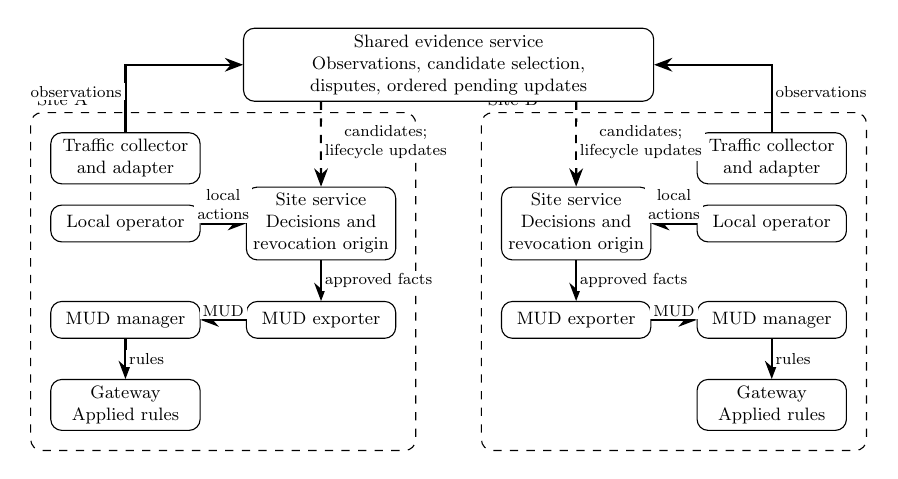
\begin{tikzpicture}[scale=0.72,transform shape,>=Stealth,
 component/.style={draw,rounded corners,align=center,font=\small,minimum height=0.65cm,text width=2.4cm,fill=white},
 flow/.style={->,thick},
 event/.style={->,thick,dashed},
 labeltext/.style={font=\footnotesize,align=center,fill=white,inner sep=1.5pt}]
\node[component,text width=7cm,minimum height=0.95cm] (evidence) at (0,0)
 {Shared evidence service\\Observations, candidate selection, disputes, ordered pending updates};
\foreach \side/\inner/\outer/\name in {a/-2.25/-5.7/A,b/2.25/5.7/B}{
 \node[component] (collector-\side) at (\outer,-1.65) {Traffic collector\\and adapter};
 \node[component] (operator-\side) at (\outer,-2.80) {Local operator};
 \node[component,minimum height=0.95cm] (site-\side) at (\inner,-2.80) {Site service\\Decisions and\\revocation origin};
 \node[component] (export-\side) at (\inner,-4.50) {MUD exporter};
 \node[component] (manager-\side) at (\outer,-4.50) {MUD manager};
 \node[component] (gateway-\side) at (\outer,-6.00) {Gateway\\Applied rules};
 \draw[flow] (operator-\side) -- node[labeltext,above]{local\\actions} (site-\side);
 \draw[flow] (site-\side) -- node[labeltext,right]{approved facts} (export-\side);
 \draw[flow] (export-\side) -- node[labeltext,above]{MUD} (manager-\side);
 \draw[flow] (manager-\side) -- node[labeltext,right]{rules} (gateway-\side);
 \begin{scope}[on background layer]
  \node[draw,dashed,rounded corners,fit=(collector-\side)(site-\side)(operator-\side)(gateway-\side)(export-\side),inner sep=0.25cm,
  label={[font=\small,anchor=south west]north west:Site \name}] {};
 \end{scope}
}
\draw[flow] (collector-a.north) |- node[labeltext,pos=0.30,left]{observations} (evidence.west);
\draw[flow] (collector-b.north) |- node[labeltext,pos=0.30,right]{observations} (evidence.east);
\draw[event] ([xshift=-2.25cm]evidence.south) -- node[labeltext,right,pos=0.47]{candidates;\\lifecycle updates} (site-a.north);
\draw[event] ([xshift=2.25cm]evidence.south) -- node[labeltext,right,pos=0.47]{candidates;\\lifecycle updates} (site-b.north);
\end{tikzpicture}
\caption{DIB's distributed architecture. Dashed boxes delimit local administrative authority. Solid arrows carry observations, local decisions, and policy output; dashed arrows carry shared candidates and lifecycle updates, which disconnected sites retrieve on reconnection. The MUD manager and gateway may be co-located, as in the OpenWrt testbed.}
\label{fig:architecture}
\end{figure*}

\subsection{Records and Operational Flow}
\label{subsec:endpoint-facts}
For device type $d$, an endpoint fact is $f=(d,e)$, where $e=(\text{direction},\text{protocol},\text{peer},\text{port})$. The peer is a Fully Qualified Domain Name (FQDN) or remote IP address. Before scoring, adapters associate observed names with addresses and normalize protocol labels. Names come from DNS records or HTTP/TLS metadata, depending on the dataset; the remaining fields come from the flow's direction, protocol, and port. Scoring uses outbound communications because the evaluated captures predominantly contain device-initiated traffic. The exporter can also generate return-flow entries.

The \emph{DIB registry} is the logical record model for shared evidence and per-site decisions. The single-registry implementation stores both in one service. In the distributed prototype, the shared evidence service holds only shared records; each site stores its own decisions (Sec.~\ref{sec:scalability-results}). Shared records contain observations, reporting sites, timestamps, and attestations. The contribute operation deduplicates submissions; attest records a positive site assessment. \emph{Local} evidence fails admission; \emph{Corroborated} evidence meets the endpoint, reporting-site, score, and dispute checks for review (Sec.~\ref{sec:scoring}). Three distinct positive attestations promote an undisputed Corroborated record to \emph{Consortium-attested}. These labels establish neither benignity nor permission to communicate.

Site-local records hold decisions and their revision history. A \textsc{query} stages an admissible fact as MonitorOnly if the site has no record, or returns its existing decision; it is therefore not a read-only operation. MonitorOnly places a proposal in the operator's review queue without generating a network rule. Local approval is recorded through \textsc{operator-commit} (a local commit), the only operation that authorizes export. Decision history records lifecycle events and the resulting state, actor, time, and reason where supplied, allowing restoration to distinguish a local veto from shared withdrawal.

\textbf{From observations to a MUD rule.} To provide an example of an observation that could become an endpoint fact, we can assume having two different sites (A and B), both having inside their network an IP Camera. In this example, the two sites report TCP traffic to \texttt{api.vendor.example} on port 443. Once admitted, the fact enters site A's review queue as MonitorOnly. An \textsc{operator-commit} moves it to Active, and the exporter emits an access-control entry (ACE) matching the destination DNS name and TCP port in the from-device access-control list (ACL), which the MUD manager resolves and installs. Site B requires its own approval. Table~\ref{tab:record-example} summarizes the outcomes of this example.
On the other side, withdrawal regenerates the site's policy, which the gateway must apply to remove installed permissions. Table~\ref{tab:transitions} specifies the recovery transitions.

\begin{table}[ht]
\centering
\caption{Illustrative records and export for the camera example. Field groups summarize stored information, not an API serialization.}
\label{tab:record-example}
\scriptsize
\begin{tabular}{@{}p{1.5cm}p{5.6cm}@{}}
\toprule
Record & Example contents \\
\midrule
Endpoint fact & (camera, out, TCP, \texttt{api.vendor.example}, 443) \\
Evidence & Reporters: sites A and B; observation timestamps and counts; computed admission score \\
Site A decision & Active after A's commit; valid approval; commit event in decision history \\
Site B decision & MonitorOnly; no approval; no exported rule \\
Site A MUD ACE & Destination DNS name \texttt{api.vendor.example}; IP protocol 6; TCP destination port 443; forwarding accept \\
\bottomrule
\end{tabular}
\end{table}

\subsection{Site-Local Authority Lifecycle}
\label{subsec:lifecycle}
\begin{figure}[t]
\centering
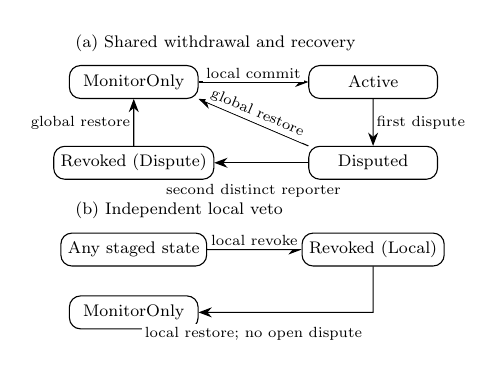
\begin{tikzpicture}[scale=0.76,transform shape,>=Stealth,
box/.style={draw,rounded corners,align=center,minimum width=2.15cm,
minimum height=0.55cm,font=\footnotesize},
lab/.style={font=\scriptsize,fill=white,inner sep=1.5pt}]
\node[font=\footnotesize,anchor=west] at (-1.1,0.65) {(a) Shared withdrawal and recovery};
\node[box] (review) at (0,0) {MonitorOnly};
\node[box] (active) at (4.0,0) {Active};
\node[box] (revoked) at (0,-1.35) {Revoked (Dispute)};
\node[box] (disputed) at (4.0,-1.35) {Disputed};
\draw[->] (review)--node[lab,above]{local commit}(active);
\draw[->] (active)--node[lab,right]{first dispute}(disputed);
\draw[->] (disputed)--(revoked);
\node[lab] at (2,-1.82) {second distinct reporter};
\draw[->] (revoked)--node[lab,left]{global restore}(review);
\draw[->] (disputed.north west)--node[lab,sloped,above]{global restore}(review.south east);
\node[font=\footnotesize,anchor=west] at (-1.1,-2.15) {(b) Independent local veto};
\node[box] (source) at (0,-2.8) {Any staged state};
\node[box] (local) at (4.0,-2.8) {Revoked (Local)};
\draw[->] (source)--node[lab,above]{local revoke}(local);
\node[box] (reviewb) at (0,-3.85) {MonitorOnly};
\draw[->] (local.south)--(4,-3.85)--(reviewb.east);
\node[lab] at (2,-4.2) {local restore; no open dispute};
\end{tikzpicture}
\caption{Recovery paths for an admitted fact. A local veto can be recorded from MonitorOnly, Active, Disputed, or Revoked (Dispute), and survives global restore. Panel (a) shows withdrawal from Active; all guards are in Table~\ref{tab:transitions}.}
\label{fig:lifecycle}
\end{figure}
Figure~\ref{fig:lifecycle} summarizes all the possible transitions that an endpoint fact $f$ can assume during its lifecycle inside a site $s$. Indeed, an endpoint fact can reside only in one of the five authorization states:
\[
S=\{\text{Absent},\text{MonitorOnly},\text{Active},\text{Disputed},\text{Revoked}\}.
\]
Revoked (Dispute) and Revoked (Local) share the state Revoked, but differ in the separately stored revocation origin.
Each local approval enters Active and creates a fresh \emph{grant}, tracked by $\texttt{grantValid}[s][f]$. Export requires both:
\begin{equation}
\begin{aligned}
\mathrm{Exportable}(s,f) \iff{}&\ \mathrm{state}(s,f)=\text{Active}\\[-2pt]
&\land\ \mathrm{grantValid}(s,f).
\end{aligned}
\label{eq:exportable}
\end{equation}

Table~\ref{tab:transitions} gives the transitions and guards, which also depend on grant validity, dispute status, and revocation origin.
\begin{table*}[ht]
\centering
\caption{Lifecycle transitions. Parenthetical labels on Revoked indicate revocation origin; slashes separate alternative source states. Repeated reports from the same site and reports after confirmed revocation add no transition. Other undefined transitions are rejected or leave the record unchanged. Retention expiry is specified here but lies outside the verified configuration and is not implemented in the prototype.}
\label{tab:transitions}
\scriptsize
\begin{tabular}{@{}llllll@{}}
\toprule
Current state & Event & Precondition & Next state & Grant valid? & Exportable? \\
\midrule
Absent & query/stage & admitted; no open dispute & MonitorOnly & no & no \\
MonitorOnly & local commit & local operator; no dispute & Active & yes, new & yes \\
MonitorOnly/Active & first dispute & valid dispute & Disputed & no & no \\
Disputed & second dispute & distinct reporting site & Revoked (Dispute) & no & no \\
Disputed/Revoked (Dispute) & global restore & authorized restore & MonitorOnly & no & no \\
Active/MonitorOnly/Disputed/Revoked (Dispute) & local revoke & local operator & Revoked (Local) & no & no \\
Revoked (Local) & local restore & no open dispute & MonitorOnly & no & no \\
MonitorOnly & retention expiry & below admission for window $W$; no local decision & Absent & no & no \\
Revoked (Local) & global restore & --- & Revoked (Local) & no & no \\
Absent & dispute & --- & Absent & no & no \\
\bottomrule
\end{tabular}
\end{table*}

Review candidates are not permanent: a MonitorOnly record with no prior operator action returns to Absent once its evidence has stayed below admission for the retention window~$W$, bounding queue growth without touching any record carrying a local decision. A local veto can be recorded from Active, MonitorOnly, Disputed, or dispute-derived Revoked. It changes only the receiving site's record and survives dispute confirmation and global restoration. Local restore remains blocked while a shared dispute is open. Once the dispute is resolved, local restore returns the record to review; export requires a fresh local commit.

\textbf{Core Invariants (I1--I3).} Under the stated identity assumptions, the lifecycle requires:
\begin{itemize}
\item \textbf{(I1) Fresh Local Authorization:} Only operator-commit by site $s$'s operator can move fact $f$ into Active and create a valid grant at that site.
\item \textbf{(I2) Site Confinement:} Local commit, revoke, and restore at site $s$ leave every peer site's records unchanged.
\item \textbf{(I3) Conservative Reversal:} A dispute invalidates grants and export eligibility at reachable sites during fan-out and at other sites upon reconciliation. Restoration requires fresh local approval and preserves independent local revocations, including those recorded at sites that missed the entire dispute/restore episode. No timing bound is imposed on reconciliation.
\end{itemize}

\textbf{Export control.} Equation~\ref{eq:exportable} gates export on current local authorization, and verification checks that commit, dispute, restore, and reconciliation maintain it across their interleavings. The mutations in Table~\ref{tab:tla} isolate failures of grant coherence, site confinement, veto preservation, and export control. Gateway application follows export, so an unreachable gateway can retain an older policy until reconnection.

\subsection{Candidate-Selection Policy}
\label{sec:scoring}
The prototype uses automatic admission to limit the proposals presented for local review. We define the admission rule, its score, and the component checks below. Table~\ref{tab:symbols} lists the parameters. The alternative selection policies evaluated in Section~\ref{sec:eval} change the review queue while retaining the same local approval and recovery rules.

\begin{table}[t]
\centering
\caption{Admission notation and operating values ($d$: device type; $e$: endpoint). $C_s$ is raw breadth unless an experiment states trust weighting.}
\label{tab:symbols}
\scriptsize
\begin{tabular}{@{}p{1.3cm}p{5.00cm}p{0.75cm}@{}}
\toprule
Symbol & Meaning & Value \\
\midrule
$ES_d$ & sites with $\ge1$ observation of device type $d$ & --- \\
$S_{d,e}$ & subset of $ES_d$ reporting endpoint $(d,e)$ & --- \\
$C_s$, $C_t$ & cross-site breadth; temporal confidence & --- \\
$m$ & minimum reporting sites (quorum) & 2 \\
$\theta$ & admission threshold & 0.65 \\
$\alpha,\beta$ & breadth / temporal weight, $\alpha+\beta=1$ & 0.6, 0.4 \\
$f_s$ & assumed per-type adversarial raw-breadth share (budget) & 0.30 \\
\bottomrule
\end{tabular}
\end{table}

\textbf{Combined rule}: Automatic staging requires endpoint eligibility, at least $m$ reporting sites, score at least $\theta$, and no unresolved dispute. The quorum counts distinct reporting identities, which need not be independent observers; Table~\ref{tab:params} justifies its value:
\begin{equation}
\begin{aligned}
\mathrm{admit}_{auto}(d,e)
={}&(A(d,e)=1)\wedge(|S_{d,e}|\ge m)\\
 &{}\wedge(score(d,e)\ge\theta)\\
 &{}\wedge\neg openDispute(d,e).
\end{aligned}
\label{eq:admitauto}
\end{equation}
Passing permits staging, not export, and does not override existing local decisions (Sec.~\ref{subsec:endpoint-facts}).

\textbf{Admission score.} With nonnegative weights $\alpha,\beta$ for breadth and temporal confidence,
\begin{equation}
score(d,e)=\alpha C_s(d,e)+\beta C_t(d,e),
\qquad \alpha+\beta=1 .
\label{eq:score}
\end{equation}

\textbf{Eligibility}: The endpoint filter sets $A(d,e)=1$ for DNS, NTP, update, or vendor-cloud communications, using port, protocol, and name-substring rules. Vendor-cloud includes any remaining FQDN, while private, reserved, and link-local IP literals are excluded. The filter selects endpoint formats and service categories, so resolved attacker domains can also qualify.

\textbf{Breadth and persistence.} Breadth $C_s=|S_{d,e}|/|ES_d|$ measures the fraction of sites observing device type $d$ that report endpoint $e$. Let $D_{d,e}$ contain the UTC observation dates of $(d,e)$ across sites, and $D_d$ the dates of all observations of $d$. With pooled observation counts $n_{d,e}$ and $n_d$, temporal confidence, used here as a measure of persistence, combines day coverage and relative frequency:
\begin{equation}
C_t=0.7\frac{|D_{d,e}|}{|D_d|}+0.3\frac{n_{d,e}}{n_d}\in[0,1].
\label{eq:ct}
\end{equation}
The 0.7/0.3 split weights day coverage above pooled volume. Counts are pooled without per-site normalization, so a single reporter can supply the whole volume term (at most $0.3\beta=0.12$ of the score) and, by reporting on every active day of $d$, the whole day-coverage term ($0.7\beta=0.28$). $C_t$ therefore enters Criterion~\ref{crit:poison-bound} only through $C_t\le1$: the split changes how much persistence a benign fact needs, not the safety bound. The split is fixed rather than tuned; we sweep only $\theta$ and $\alpha$ (Sec.~\ref{sec:sensitivity-results}).

\textbf{Parameter derivation.} The weights are not free. Since $\alpha+\beta=1$, only $(\alpha,\theta)$ remain, and a single quantity links them to protection, the \emph{breadth margin}
\begin{equation}
f^\star=\frac{\theta-\beta}{\alpha}=1-\frac{1-\theta}{\alpha}.
\label{eq:fstar}
\end{equation}
Given eligibility and quorum, Eq.~\ref{eq:score} admits a fact whose reporters hold raw breadth share $c$ and whose persistence is $C_t$ if and only if
\begin{equation}
c\ \ge\ f^\star+\frac{\beta}{\alpha}\,(1-C_t).
\label{eq:benignbreadth}
\end{equation}
With $C_t=1$ this reduces to $c\ge f^\star$, so $f^\star$ has two readings: it is the largest adversarial share the score alone can absorb, and the smallest breadth at which a benign fact can pass even with perfect persistence. The ratio $\beta/\alpha$ sets how much additional breadth a persistence deficit costs. Raising $\theta$ at fixed $\alpha$ raises $f^\star$; raising $\alpha$ at fixed $\theta$ raises $f^\star$ and lowers $\beta/\alpha$. A larger $f^\star$ gives more protection but requires more breadth from benign facts (less recall); Sec.~\ref{sec:sensitivity-results} measures this trade-off. At $(\alpha,\theta)=(0.6,0.65)$, $f^\star=5/12\approx0.417$ and $\beta/\alpha=2/3$: a fact reported on every active day of $d$ but with negligible volume share ($C_t\approx0.7$) needs $c\ge0.617$, i.e., seven of ten eligible sites.

\begin{criterion}[Admission design constraint, raw breadth]
\label{crit:poison-bound}
If malicious contributors hold at most raw breadth share $f_s$ (the unweighted share $|S_{d,e}|/|ES_d|$) of the eligible population and an endpoint fact is reported only by them, then $C_s\le f_s$ and $C_t\le1$, so
\begin{equation}
score(d,e)\le\alpha f_s+\beta
=1-\alpha(1-f_s).
\label{eq:poisonbound}
\end{equation}
Requiring this upper bound to fall strictly below $\theta$ constrains the parameters to $\alpha>(1-\theta)/(1-f_s)$, equivalently $f_s<f^\star$ (Eq.~\ref{eq:fstar}).
\end{criterion}

At $\theta=0.65$ and $f_s=0.30$ this requires $\alpha>0.5$. Choosing $\alpha=0.6$ gives an upper bound of 0.58 and rejects adversary-only evidence for raw-breadth shares below $5/12$. The guarantee holds per device type, and the bound is a supremum: it is approached only if $C_t\to1$, which requires the adversary to cover every active day of $d$ and dominate its volume while honest observations of $d$ exist, so a share of exactly $5/12$ is also rejected. In counts, with $K$ adversarial and $h$ honest reporting sites for $d$, the score alone rejects every adversary-only fact if $K\le\frac{\theta+\alpha-1}{1-\theta}\,h$, that is, $K\le\frac57h$ at the operating point; above this ratio admission becomes possible, depending on the adversary's persistence and volume. Three colluders thus require at least five honest sites at the margin and at least seven at the declared share $f_s=0.30$. Device types observed by few sites are therefore the binding case: with $h\le2$, the smallest non-zero adversarial share is $1/3>f_s$, and the quorum $m=2$, not the score, rejects single-source facts.

\textbf{Why $f_s=0.30$.} Only one statement about $f_s$ is derived: Criterion~\ref{crit:poison-bound} protects every share below $f^\star$, so any budget $f_s<f^\star$ is consistent with the operating point. The value $0.30$ is an assumption, a planning budget rather than a measured prevalence, chosen on three grounds. First, it leaves a margin of $f^\star-f_s=7/60\approx0.117$, so a share that exceeds the budget by less than this margin is still rejected. Second, it lies below the $1/3$ fault fraction tolerated by classical Byzantine agreement ($n\ge3f+1$)~\cite{lamport1982byzantine,castro1999pbft}; this is an order-of-magnitude reference only, because the DIB guard is a threshold on reporting share, not an agreement protocol. Third, the budget covers two populations with different empirical anchors. For colluding members (A2), the share is a governance property of the consortium, for which the Byzantine bound is the natural reference. For honest sites that report traffic of compromised devices (A1), it is a prevalence, and measurement studies give no per-type value to match: Mirai peaked at about 600{,}000 infections without a per-type share~\cite{mirai}; 1.3\% of devices in homes seen scanning (0.37\% of homes) were compromised through an EternalBlue backdoor, and scan data rarely reveal compromise~\cite{kumar2019allthings}; and 28.25\% of 1{,}362{,}906 deployed devices had at least one known vulnerability, with per-vendor rates from below 0.5\% to 100\%~\cite{zhao2022largescale}. Vulnerable is not compromised, so $0.30$ is conservative against measured compromise and of the same order as measured vulnerability prevalence.

A probabilistic reading makes the budget explicit. If $n$ devices of type $d$ share a site and each is compromised independently with probability $p$, the site reports compromised traffic with probability $q=1-(1-p)^n$; for $p=0.10$ and $n=4$, $q=0.34$. If each of the $N_d$ sites observing $d$ is adversarial independently with probability $q$, admission of an adversary-only fact becomes possible once $K\ge\lceil5N_d/12\rceil$. For $q=0.10$ this event has probability $1.6\times10^{-3}$ at $N_d=10$, $6.0\times10^{-5}$ at $N_d=20$, and $3.7\times10^{-9}$ at $N_d=50$; for $q=0.30$ it is 0.15, 0.11, and 0.048. The declared budget covers $K\le\lfloor0.30N_d\rfloor$ (three sites at $N_d=10$), so $f_s$ is better read as a quantile of the compromise distribution than as its mean. Correlated sites (shared firmware, shared vendor cloud) make the independent tail an underestimate.

\textbf{Sybil-aware variants.} Raw breadth counts identities, so fabricated ones inflate it. Trust weighting replaces $C_s$ with
\[
C_s^{trust}=\frac{\sum_{i\in S_{d,e}}w_i}{\sum_{i\in ES_d}w_i},\qquad w_i=\min(1,b_i/b_{ref}),
\]
Here, $b_i$ counts site $i$'s distinct contributed facts across device types, and $b_{ref}$ is their median in a frozen clean snapshot. Only $b_{ref}$ is frozen, so current $b_i$ includes new identities and padding. Clustering instead joins sites at Jaccard endpoint-set similarity $\ge0.8$ and computes breadth over the connected components. Sec.~\ref{subsec:security-analysis} discusses which guarantee applies to each variant, and Sec.~\ref{sec:sensitivity-results} compares them under identity inflation.

\textbf{Parameter rationale.} Table~\ref{tab:params} states the basis of each value and the effect of a change. Safety fixes only the constraint $f^\star>f_s$; the operating point keeps one further degree of freedom, $\beta/\alpha$, which affects recall but not protection. The $\theta,\alpha$ sweep (Sec.~\ref{sec:sensitivity-results}) characterizes this trade-off and was not used to select the operating point.

\begin{table}[t]
\centering
\caption{Admission parameters. D: derived; A: assumed; U: untuned.}
\label{tab:params}
\scriptsize
\begin{tabular}{@{}p{0.95cm}p{3.35cm}p{2.85cm}@{}}
\toprule
Param. & Basis & Effect of a change \\
\midrule
$f_s=0.30$ & A: budget below $f^\star$ and below $1/3$; prevalence anchors (Sec.~\ref{sec:scoring}) & not used by the score; needs $f^\star>f_s$ \\
$\theta=0.65$ & D with $\alpha$: Criterion~\ref{crit:poison-bound} needs $\theta>\beta+\alpha f_s=0.58$. \nongiust{0.65 within $(0.58,1)$} & higher: larger $f^\star$, lower recall; $\le0.58$ voids the criterion \\
$\alpha=0.6$ & D: $\alpha>(1-\theta)/(1-f_s)=0.5$. \nongiust{0.6 within $(0.5,1]$} & higher: larger $f^\star$, persistence matters less; $\le0.5$ voids the criterion \\
$\beta=0.4$ & D: $\beta=1-\alpha$ & as for $\alpha$ \\
$m=2$ & D: with $h\le1$ honest observers the score alone can admit a single reporter & $m=1$ admits single colluders; $m=3$ rejects every fact with two reporters \\
0.7/0.3 & U: fixed, not swept; does not affect Criterion~\ref{crit:poison-bound}. \nongiust{0.7/0.3} & changes the persistence a benign fact needs (Eq.~\ref{eq:benignbreadth}) \\
\bottomrule
\end{tabular}
\end{table}

\subsection{Security Analysis}
\label{subsec:security-analysis}
Table~\ref{tab:threats} relates the mechanisms above to the goals and threats of Sec.~\ref{sec:threat}.

\begin{table}[t]
\centering
\caption{Threats, goal at risk, and DIB's response. G3 holds under every threat, given AS1, AS4, and AS5.}
\label{tab:threats}
\scriptsize
\begin{tabular}{@{}p{1.45cm}p{0.95cm}p{4.65cm}@{}}
\toprule
Threat & Goal & Response; residual risk \\
\midrule
A1 & G2 & counted in $f_s$; eligibility rejects IP-literal peers, but resolved attacker names can enter review \\
A2 within AS2 & G2 & quorum and Criterion~\ref{crit:poison-bound} (raw breadth) \\
A2 beyond AS2 & G2 & no guarantee; trust weighting and clustering are heuristics \\
A3 & G1, G2 & identical evidence; requires local review or out-of-band information \\
A4 & avail. & withdrawal creates no authorization; restoration needs the administrator and a fresh commit \\
Disconnection & G3 & ordered pending update applied on reconnection; no time bound \\
Faulty evidence service & G2 & holds no local authorization state \\
\bottomrule
\end{tabular}
\end{table}

\textbf{G3.} G3 follows from the lifecycle guards (I1--I3, Eq.~\ref{eq:exportable}), which hold for any content of shared evidence; A1--A4 therefore cannot create local authorization under AS1, AS4, and AS5. A faulty evidence service can delay withdrawal or issue unfounded disputes and restorations, but a restoration returns records to MonitorOnly (Table~\ref{tab:transitions}), so it cannot make a fact exportable either; sites ignore any update whose target state differs from Table~\ref{tab:transitions}. A site that misses an episode applies the latest ordered update on reconnection, without a time bound (AS6). The prototype enforces them with a two-phase commit that re-reads the evidence before a record becomes Active (Sec.~\ref{sec:lifecycle-results}).

\textbf{G2.} G2 is the guarantee of Criterion~\ref{crit:poison-bound} and holds only under AS2 and with raw breadth. Under trust weighting, an adversary-only fact has $C_s^{trust}=W$, where $W=\sum_{i\in S_{d,e}}w_i/\sum_{i\in ES_d}w_i$ is the adversaries' weighted share, so the same algebra rejects it whenever $W<f^\star$. The weights, however, grow with $b_i$, which counts the facts that site $i$ itself contributes: a member that contributes many facts reaches full weight while honest sites with fewer contributions keep lower weights, so $W$ can exceed the raw share, and a fact can pass with a raw share below $f^\star$. Results obtained with trust weighting are therefore not covered by Criterion~\ref{crit:poison-bound}, and clustering has no analogous bound. Fabricated identities beyond AS2 and A1 traffic reported by more than a fraction $f_s$ of observers fall outside G2. Admission failure creates a false proposal, not a rule (G3).

\textbf{G1, A3, and A4.} Candidate selection gives no guarantee about intent: under A3, separating legitimate from malicious change requires local review or out-of-band information, and Active facts that later fail admission keep their approval and receive a review flag. A4 affects availability only: withdrawal removes rules but cannot install them, and suspending a fact after one or after two distinct reporters trades withdrawal speed for robustness to a single false notice (Sec.~\ref{sec:suspension-policy}).

\section{Implementation and Evaluation Method}
\label{sec:impl}
The distributed prototype separates shared evidence from site-local decisions into distinct services (Sec.~\ref{sec:scalability-results}). Each service is a Python/FastAPI process with its own SQLite database. Opt-in mutual TLS maps the client certificate's SAN URI to a site and role; without it, endpoints are unauthenticated.

For enforcement, unmodified osMUD \texttt{852918e} runs in a privileged OpenWrt 23.05.5 container; on each change the harness exports the site's MUD file and restarts osMUD, and polls state, nftables rules, and TCP connections every 10--50~ms on one clock. Exports are unsigned and signature validation is disabled.

Candidate-selection experiments use three traffic datasets. UNSW-IoTraffic~\cite{sivanathan2019classifying} supplies 27 device types and 28 traffic-derived reference profiles; its single capture is shuffled and partitioned round-robin into ten pseudo-sites (seed 42 unless stated). Mon(IoT)r~\cite{moniotr} provides US and UK captures after collapsing VPN variants; YourThings~\cite{alrawi2019yourthings} adds a third deployment for cross-lab comparisons (Sec.~\ref{sec:loo-results}). We retain device-initiated flows with a port and global peer or public name. UNSW associates IPs with same-site HTTP Host and TLS Server Name Indication (SNI) within 24 hours; Mon(IoT)r uses cumulative DNS.

Using these observations, we assess sharing by comparing receiver-only evidence (\emph{local-only}) with all pooled facts (\emph{pooled union}). Successively adding a two-reporter quorum, the score threshold, and endpoint eligibility isolates filtering effects, while \emph{ranked union} selects the highest-scoring pooled facts at matched review budgets.

We then test robustness with captured and synthetic inputs. The A1 replay injects 165 malicious observations forming 59 endpoint facts at $k=1,\ldots,10$ pseudo-sites, using \emph{frequency filtering} ($n_{d,e}\ge2$ pooled observations) as a baseline. Further tests inject fabrications, resolved-name and port masquerading, Sybil identities (200--3,200 over 20--400 days), and synthetic rollouts, with fabricated endpoint sets diversified by 0/10/25/50\% of a baseline pool. For identity inflation, \emph{reputation-weighted voting (RWV)} provides a comparison requiring weighted support above 0.65, with frozen pre-attack weights and weight 0.1 for unseen identities.

To measure agreement with reference behavior, we match predictions on device, direction, normalized protocol, peer, and port, treating port 0 and unknown protocol as wildcards and CIDR ranges by membership. Micro metrics pool true/false positives and negatives; UNSW macro metrics average over its 28 reference profiles.



For reproducibility, the anonymized repository supplied with the submission contains configurations, input hashes, adapters, sampling details, generated MUD files, gateway states and probes, TLA+ specifications and logs, matched ablations, parameter and identity-inflation grids, and regression evidence. 

\section{Evaluation}
\label{sec:eval}
We assess whether DIB preserves local authorization during withdrawal and recovery, how fast both are under delay and loss, and what candidate selection achieves on captured traffic. Withdrawal and recovery timing run ten site services and an evidence service in Docker on one 16-vCPU KVM node, with \texttt{tc netem} on every container; gateway timing runs on a separate shared 16-core host with \texttt{netem} on the evidence service's link only. Hypotheses were fixed before the runs. Gateway timing predates the target-state guard (Sec.~\ref{subsec:security-analysis}); a smoke run after it matched.

\subsection{Authorization and Recovery}
\label{sec:lifecycle-results}
The TLA+ model represents three sites and two facts, distinguishing the dispute opener, confirmer, and bystander. Exhaustive exploration of 4,311,852 states finds no violation of I1--I3 or the export checks: only local commits create fresh authorization, export requires it, and disputes invalidate it without affecting unrelated facts. With one of three sites disconnected, one fact, and local revoke and restore enabled, 48,960 states show no violation. A model of the implemented non-atomic query and commit protocol (two sites, one fact) explores 402,633,492 states with three evidence events and partitions without violations; removing any of its five corrections produces one. Adding failed evidence reads, abandoned reconcile runs, and site crash with restart cleanup, safety holds in separate configurations: three events with a failed read and a crash (154,363,430 states), three sites (712,287,745), and partitions, lost deliveries, quorum two, and two facts. Removing the cleanup produces a violation. These checks are exhaustive only within their finite configurations; they do not cover gateway timing, concurrent requests per site, three-event convergence with failures, or linearizability.

To identify which safeguards prevent failures, we remove six lifecycle guards in separate model variants, M1--M6. Each produces a distinct authorization failure involving grant handling, site confinement, revocation origin, or export control (Table~\ref{tab:tla}). A separate model of the mTLS authorization rules, extracted from the service code, checks role and site confinement; its ten base configurations find no counterexample and six mutants each violate the property they remove. It assumes mutual TLS and one identity per certificate.

\begin{table}[t]
\centering
\caption{Guard-removal mutations M1--M6 and their counterexamples. A separate control with operator-commit disabled leaves 2,076,196 reachable states, none Active.}
\label{tab:tla}
\scriptsize
\begin{tabular}{@{}p{0.35cm}p{2.05cm}p{1.85cm}p{1.95cm}@{}}
\toprule
ID & Property & Guard removed & Counterexample \\
\midrule
M1 & Grant coherence & restore recreates grant & authorization without commit \\
M2 & I2 site confinement & cross-site commit & remote commit alters $s'$ \\
M3 & Export requires Active & disputed export & ACE emitted while Disputed \\
M4 & Dispute suspends everywhere & local-restore ignores open dispute & site escapes live dispute \\
M5 & I2 local-revoke confinement & local-revoke fans out & remote site's record changes \\
M6 & I3 global restore preserves local revoke & restore ignores revocation origin & local veto erased \\
\bottomrule
\end{tabular}
\end{table}

The registry tests exercise these rules through one- and two-dispute episodes, repeated restoration, and local vetoes recorded before or during withdrawal. Among three restoration policies, only DIB prevents export of a disputed fact without a new commit while preserving every local veto: reusing approvals exports the fact at 12 of 18 non-vetoing sites, and resetting all records to review erases all six vetoes. In 210 gateway episodes with mutual TLS (100 \emph{lan}, 50 \emph{wan}, 50 \emph{degraded}, 10 with a veto), every dispute withdrew its fact and spared an unrelated one: medians of 24~ms to invalidate the site approval (0.42, 1.02~s), 0.38~s to refuse new connections, and 5.49~s to install the policy (5.88, 6.50~s), mostly osMUD's restart, which also paused the unrelated fact for 5.1~s. Established connections were never cut. Restore alone never re-enabled access; a fresh commit did; vetoes survived.

\subsection{Recovery After a Site Restart}
\label{sec:scalability-results}
When a site becomes unreachable, the service retains only the latest pending target for each fact and applies it on reconnection through the same idempotent path, using a monotonic per-fact sequence number; a restore target therefore invalidates an old Active approval even if the preceding dispute never reached the site. We kill one site while $k$ distinct endpoints are each disputed, confirmed, and restored, restart it, and measure convergence from its start (a site that stays up while partitioned is not measured), for $k=1$, 10, and 50 (50 at \emph{lan} only), reconciliation interval $T\in\{5,15\}$~s, with and without mutual TLS, in three network profiles (\emph{lan}, \emph{wan}: 80~ms and 1\% loss per direction, \emph{degraded}: 200~ms and 5\%). Each of the 28 cells has 30 trials (two series of 10 and 20 trials with different seeds, pooled). The pre-registered bound is $1.5+0.1T+\max(5,D_{run})$~s, 7.0--8.6~s.

The median convergence is 0.6--1.4~s at \emph{lan}, including 50 missed episodes (0.7--1.4~s), 1.4--2.1~s at \emph{wan}, and 2.4--4.1~s at \emph{degraded}; it stays below the bound in all 28 cells. Six of 840 trials were excluded (five refused setups, one non-empty queue; 16 setup retries); in the other 834 the restarted site ends with every fact in MonitorOnly. At \emph{degraded}, 3 of 234 trials exceed the bound (by 0.1 to 4.0~s); in the one we traced, with mutual TLS, the first reconciliation attempt timed out in the TLS handshake (5~s) and the second succeeded.

\subsection{Withdrawal Under Emulated Network Delay and Loss}
\label{sec:netem-results}
A generator on the node sends a dispute and timestamps each site's \texttt{/apply\_fanout} log line with the clock that stamped the dispute, so the withdrawal time of the last site excludes the response path. Each cell crosses sequential and concurrent fan-out (1 or 10 sites at a time) with the presence (C) or absence (D) of mutual TLS; the \emph{degraded} profile ($R=400$~ms round trip, 5\% loss per direction) has two replicas of 50 episodes per cell, run on a deployment whose containers were verified to execute the evaluated service.

We explain the delays with a delivery-cost model that has no fitted parameter: an attempt is a TCP handshake, with mutual TLS a TLS round trip and the client certificate flight, and a two-segment request; a lost segment is retransmitted after $R+\max(2R,0.2)$~s, which for $R\ge0.2$~s exceeds the 1~s per-phase timeout, so one loss fails the attempt; the periodic reconciliation then brings each site to the disputed state. The model was checked out of sample in a network-namespace testbed (six conditions, within 1.7 points) and on the deployment (Table~\ref{tab:netem}). Without mutual TLS it predicts the share of late deliveries per site within 3.4 points in five conditions (two \emph{degraded} replicas and four further conditions with $R=0.12$--0.30~s and loss 4--8\%) and the median of the last site within 9\% under sequential fan-out. With mutual TLS it is a lower estimate: the measured share exceeds it by 3--7 points in four of five conditions. In the testbed, sequential fan-out took 3.1--7.1 times the median withdrawal time of concurrent fan-out, and every site reached the disputed state in 3,280 episodes with loss; the service therefore fans out concurrently by default.

\begin{table}[t]
\centering
\caption{Withdrawal at \emph{degraded}: median time of the last site (ms) and share of late deliveries per site, delivery-cost model against two replicas (R1, R2) of 50 episodes. Late: more than 0.75 round trips beyond the lossless time.}
\label{tab:netem}
\scriptsize
\begin{tabular}{@{}llrrr@{}}
\toprule
Cell & Quantity & Model & R1 & R2 \\
\midrule
D, 10 sites & last site (ms) & 2000 & 1621 & 2012 \\
C, 10 sites & last site (ms) & 2800 & 2823 & 2821 \\
D, 1 site & last site (ms) & 10600 & 11517 & 10774 \\
C, 1 site & last site (ms) & 17200 & 17215 & 16701 \\
D, 10 sites & late share & 0.179 & 0.189 & 0.204 \\
C, 10 sites & late share & 0.280 & 0.314 & 0.340 \\
\bottomrule
\end{tabular}
\end{table}

\subsection{Suspension Policy and Availability}
\label{sec:suspension-policy}
With immediate suspension, one member's requests withdraw the disputed facts across ten sites and take exports from the approved ACEs to zero, while the services keep answering; under two-reporter suspension the first report is retained and the second opens the dispute, duplicate reports add no votes, and local vetoes recorded during withdrawal survive restoration with fresh commits required for export. One identity's 100 disputes withdrew 1,000 site records in a median 5.2~s, cutting concurrent read throughput from 662 to 228 operations/s.

\subsection{Candidate Selection on Captured Traffic}
\label{sec:utility-results}
In UNSW, only 55 of the 564 reference ACEs across 28 profiles remain observable after address filtering. DIB stages 36 of the observable ACEs, retaining 65.5\% of observable behavior. Pooling helps at cold start (macro F1 $0.112\pm0.002$ for ten pseudo-sites after 30 days, against $0.022\pm0.005$ for one), but this reflects a larger sample, not agreement across independent networks: the pseudo-sites are shards of one capture.

\subsubsection{Candidate Review Volume}
\label{sec:workload-results}
The independent Mon(IoT)r US and UK captures share 26 device types. Of 24,886 distinct pooled facts, 24,046 occur at only one site and 840 at both, so the two-site quorum produces the largest reduction; the score threshold narrows the queue to 697 facts and endpoint eligibility to 462: 98.1\% fewer than pooling and 33.7\% fewer than quorum with scoring.

\subsubsection{Proposals for a New Receiving Site}
\label{sec:loo-results}
A new receiving site must not use its own observations to select proposals, so we exclude the receiver from reporter sets and counts. YourThings (YT)~\cite{alrawi2019yourthings} supplies a third deployment, and a fixed six-entry label mapping aligns the device types present in all three. Each receiver uses the other two deployments as sources (Table~\ref{tab:threelab}); precision, recall, and F1 measure macro per-device agreement with receiver-observed endpoints.

\begin{table}[t]
\centering
\caption{Matched cold-start ablation: each receiver uses the other two deployments as sources. Q=two-site quorum; S=score with raw breadth ($\alpha=0.6$, $\beta=0.4$, $\theta=0.65$, no trust weights); C=endpoint eligibility; N=candidates; Cov.=device coverage; P/R/F1=macro agreement with receiver traffic over six device types. Full-DIB 95\% F1 CIs (US/UK/YT): [.033,.198]/[.044,.186]/[.116,.384].}
\label{tab:threelab}
\scriptsize
\begin{tabular}{@{}llrrrrr@{}}
\toprule
Receiver & Filter & N & Cov. & P & R & F1 \\
\midrule
US & Union & 1005 & 100\% & .322 & .358 & .327 \\
 & Q & 42 & 83.3\% & .750 & .079 & .139 \\
 & QS & 40 & 83.3\% & .750 & .076 & .135 \\
 & DIB (QSC) & 36 & 83.3\% & .750 & .065 & .116 \\
\midrule
UK & Union & 767 & 100\% & .279 & .449 & .320 \\
 & Q, QS & 48 & 83.3\% & .745 & .078 & .138 \\
 & DIB (QSC) & 43 & 83.3\% & .784 & .064 & .115 \\
\midrule
YT & Union & 1387 & 100\% & .059 & .334 & .095 \\
 & Q & 177 & 100\% & .173 & .282 & .208 \\
 & QS & 146 & 100\% & .257 & .282 & .268 \\
 & DIB (QSC) & 107 & 100\% & .286 & .223 & .247 \\
\bottomrule
\end{tabular}
\end{table}

DIB reduces candidate counts by 96.4\% at US, 94.4\% at UK, and 92.3\% at YT and raises precision to 0.75/0.78/0.29 from 0.32/0.28/0.06 for the pooled union. The reduction trades coverage for review effort: the union contains more receiver-observed endpoints and has the higher macro F1 at US and UK, but needs 5.46/4.31/28.31 inspected entries per receiver-observed endpoint, against 1.03/1.16/2.89 for DIB. Admission and ordering serve different purposes: ranking limits review to a budget, whereas admission excludes adversary-only evidence under the raw-breadth Criterion~\ref{crit:poison-bound}; we recommend threshold-then-rank. These comparisons describe filter behavior on the selected captures; only six device types are common to the three deployments and the 95\% F1 intervals overlap across receivers.

\subsection{Adversarial Observations and Fabricated Evidence}
\label{sec:security-results}
We inject captured malicious traffic and fabricated reports into the ten UNSW pseudo-sites, whose partition fixes the reporting population and lets us control the raw malicious breadth share $f_s$ of Criterion~\ref{crit:poison-bound}. This does not establish reporter independence in a real consortium; that remains a governance assumption (Sec.~\ref{subsec:trust}). DIB stages none of the 59 captured A1 facts, which pooled union and frequency filtering stage in full. At $f_s=0.30$ the largest score passing quorum is 0.562 over 120 days, below $\theta$, and an exhaustive worst case with raw breadth reaches 0.579, within the bound of 0.58. The guarantee is conditional: it holds up to $f_s=0.30$, and replacing IP literals with resolvable names raises admission from 0/150 to 21/150 configurations; a fabrication at $f_s=0.50$ reaches 0.663 (Sec.~\ref{sec:sensitivity-results} treats identity inflation). \subsubsection{Parameter Sensitivity, Identity Inflation, and Drift}
\label{sec:sensitivity-results}
The operating point chosen from the adversarial bound is not the one that maximizes traffic agreement: sweeping $\theta\in[0.50,0.80]$ and $\alpha\in[0.4,0.9]$ on Mon(IoT)r yields a best macro F1 of 0.071, against 0.054 at the chosen setting. Identity inflation deliberately violates the malicious-share assumption: raw counting admits the fabrication in 45 of 48 representative configurations, trust weighting and clustering reject them, and padding fabricated identities with real endpoints defeats clustering at the extreme (score 0.905).

\section{Discussion}
\label{sec:discussion}

Recovery requires approval validity and revocation origin, whether represented through states or history. The mutations (Table~\ref{tab:tla}) and the restoration-policy ablation (Sec.~\ref{sec:lifecycle-results}) expose failures when this information or its checks are omitted. The review process still requires evaluation with operators.

Candidate selection can adapt without changing local authorization or recovery. Quorum accounts for most queue reduction at US/UK; ordering explains the advantage over unranked pooling. Threshold-then-rank suits deployments that maintain the bounded raw-breadth share assumption of Criterion~\ref{crit:poison-bound}. Trust weighting and clustering mitigate tested identity inflation but fail under padding. Ranked union yields at least as many receiver-observed endpoints at matched budgets (35/39/40 vs.\ 35/37/37), but no tested policy establishes benignity or necessity. Review capacity should inform the retention window $W$, whose practical value remains open.

Local control does not eliminate withdrawal's availability costs. One reporter can interrupt service under immediate suspension; requiring two preserves permissions until corroboration but delays withdrawal if no second report arrives. Both policies remain vulnerable to collusion, and the prototype lacks dispute rate limits and reputation penalties. Unreachable gateways can retain stale rules until reconnection, with no withdrawal deadline meanwhile. A site can record a veto offline, but its local restore reads the evidence service and is refused while it is unreachable, unlike in the model.


The shared evidence service is a single point of failure for candidate flow and withdrawal propagation, and every site's commit reads it twice. It holds no local authorization state: failure can delay withdrawal but cannot grant or revoke local permissions; replication remains a deployment concern. Experiments emulate delay and loss on a single host and use no production workload; finite models assume authenticated callers; gateway tests disable signature validation, and withdrawal there stops only new connections. Deployment requires the authentication, roles, and signing integration in Sec.~\ref{subsec:trust}.

The pseudo-site partition and six-type alignment restrict generalization. Coverage of fleets using these mechanisms remains unverified.


\section{Conclusion}
\label{sec:conclusion}
This paper presented DIB for managing locally authorized MUD policies from shared IoT observations. Bounded model checks and mutations assess its lifecycle, OpenWrt/osMUD episodes measure withdrawal at the gateway, and outage experiments show that one collapsed update preserves vetoes and invalidates stale approvals. Future work will evaluate operator review, mechanisms to bound gateway withdrawal time, and recovery of the shared evidence service.

\setlength{\IEEEbibitemsep}{0pt}
\begin{thebibliography}{00}
\footnotesize

\bibitem{mirai} M. Antonakakis \emph{et al.}, ``Understanding the Mirai Botnet,'' in
\emph{Proc. 26th USENIX Security Symp.}, 2017, pp. 1093--1110.

\bibitem{lamport1982byzantine} L. Lamport, R. Shostak, and M. Pease, ``The Byzantine Generals Problem,'' \emph{ACM Trans. Program. Lang. Syst.}, vol. 4, no. 3, pp. 382--401, 1982.

\bibitem{castro1999pbft} M. Castro and B. Liskov, ``Practical Byzantine Fault Tolerance,'' in \emph{Proc. 3rd USENIX Symp. Operating Systems Design and Implementation (OSDI)}, New Orleans, LA, USA, Feb. 1999, pp. 173--186.

\bibitem{kumar2019allthings} D. Kumar, K. Shen, B. Case, D. Garg, G. Alperovich, D. Kuznetsov, R. Gupta, and Z. Durumeric, ``All Things Considered: An Analysis of IoT Devices on Home Networks,'' in \emph{Proc. 28th USENIX Security Symp.}, 2019, pp. 1169--1185.

\bibitem{zhao2022largescale} B. Zhao, S. Ji, W.-H. Lee, C. Lin, H. Weng, J. Wu, P. Zhou, L. Fang, and R. Beyah, ``A Large-Scale Empirical Study on the Vulnerability of Deployed IoT Devices,'' \emph{IEEE Trans. Dependable Secure Comput.}, vol. 19, no. 3, pp. 1826--1840, May/Jun. 2022.

\bibitem{rfc8520} E. Lear, R. Droms, and D. Romascanu, ``Manufacturer Usage Description
Specification,'' RFC 8520, IETF, Mar. 2019.

\bibitem{clearasmud} A. Hamza, D. Ranathunga, H. Habibi Gharakheili, M. Roughan, and
V. Sivaraman, ``Clear as MUD: Generating, Validating and Applying IoT Behavioral
Profiles,'' in \emph{Proc. ACM SIGCOMM Workshop IoT S\&P}, 2018.

\bibitem{sivanathan2019classifying} A. Sivanathan \emph{et al.}, ``Classifying IoT Devices
in Smart Environments Using Network Traffic Characteristics,'' \emph{IEEE Trans. Mobile
Comput.}, vol. 18, no. 8, pp. 1745--1759, 2019.

\bibitem{hamzatdsc} A. Hamza \emph{et al.}, ``Verifying and Monitoring IoTs Network
Behavior Using MUD Profiles,'' \emph{IEEE Trans. Dependable Secure Comput.}, vol. 19, no.
1, pp. 1--18, 2022.

\bibitem{mudflow} A. Hamza, H. Habibi Gharakheili, T. A. Benson, and V. Sivaraman,
``Detecting Volumetric Attacks on IoT Devices via SDN-Based Monitoring of MUD Activity,''
in \emph{Proc. ACM SOSR}, 2019.

\bibitem{CornoMannella2023GatewayMUD} F. Corno and L. Mannella, ``A Gateway-based MUD
Architecture to Enhance Smart Home Security,'' in \emph{Proc. SpliTech}, 2023, pp. 1--6.

\bibitem{osmud} osMUD Project, ``osMUD: Open Source MUD Manager,''
\url{https://osmud.org}. (Accessed Jul. 24, 2026.)

\bibitem{hernandezramos2021mudreview} J. L. Hern\'andez-Ramos, S. N. Matheu,
A. Feraudo, G. Baldini, J. Bernal Bernabe, P. Yadav, A. Skarmeta, and
P. Bellavista, ``Defining the Behavior of IoT Devices Through the MUD Standard:
Review, Challenges, and Research Directions,'' \emph{IEEE Access}, vol. 9,
pp. 126265--126285, 2021.

\bibitem{matheu2019mudtesting} S. N. Matheu, J. L. Hern\'andez-Ramos, S. P\'erez,
and A. F. Skarmeta, ``Extending MUD Profiles Through an Automated IoT Security
Testing Methodology,'' \emph{IEEE Access}, vol. 7, pp. 149444--149463, 2019.

\bibitem{ndiot2019} T. D. Nguyen \emph{et al.}, ``D\"IoT: A Federated Self-learning Anomaly
Detection System for IoT,'' in \emph{Proc. IEEE ICDCS}, 2019, pp. 756--767.

\bibitem{vasilomanolakis2015collaborative} E. Vasilomanolakis, S. Karuppayah,
M. M\"uhlh\"auser, and M. Fischer, ``Taxonomy and Survey of Collaborative Intrusion
Detection,'' \emph{ACM Comput. Surv.}, vol. 47, no. 4, Art. 55, 2015.

\bibitem{colearn} A. Feraudo, P. Yadav, V. Safronov, D. A. Popescu, R. Mortier,
S. Wang, P. Bellavista, and J. Crowcroft, ``CoLearn: Enabling Federated Learning
in MUD-Compliant IoT Edge Networks,'' in \emph{Proc. ACM EdgeSys}, 2020,
pp. 25--30.

\bibitem{mudscope} L. Morgese Zangrandi, T. van Ede, T. Booij,
S. Sciancalepore, L. Allodi, and A. Continella, ``Stepping out of the MUD:
Contextual Threat Information for IoT Devices with Manufacturer-Provided
Behavior Profiles,'' in \emph{Proc. ACSAC}, 2022, pp. 467--480.

\bibitem{wagner2016misp} C. Wagner, A. Dulaunoy, G. Wagener, and A. Iklody, ``MISP: The
Design and Implementation of a Collaborative Threat Intelligence Sharing Platform,'' in
\emph{Proc. ACM WISCS}, 2016, pp. 49--56.

\bibitem{stix21} OASIS CTI TC, ``STIX Version 2.1,'' OASIS Standard, Jun. 2021.

\bibitem{eigentrust} S. D. Kamvar, M. T. Schlosser, and H. Garcia-Molina, ``The EigenTrust
Algorithm for Reputation Management in P2P Networks,'' in \emph{Proc. WWW}, 2003.

\bibitem{trustsurvey} A. J\o{}sang, R. Ismail, and C. Boyd, ``A Survey of Trust and
Reputation Systems for Online Service Provision,'' \emph{Decision Support Systems}, vol.
43, no. 2, pp. 618--644, 2007.

\bibitem{pbnm} M. Sloman, ``Policy Driven Management for Distributed Systems,'' \emph{J.
Netw. Syst. Manage.}, vol. 2, no. 4, pp. 333--360, 1994.

\bibitem{rfc9315} A. Clemm, L. Ciavaglia, L. Z. Granville, and J. Tantsura,
``Intent-Based Networking: Concepts and Definitions,'' RFC 9315, IETF, Oct. 2022.

\bibitem{alshaer2004firewall} E. Al-Shaer and H. Hamed, ``Modeling and Management of
Firewall Policies,'' \emph{IEEE Trans. Netw. Serv. Manage.}, vol. 1, no. 1, pp. 2--10,
Apr. 2004, doi: 10.1109/TNSM.2004.4623689.

\bibitem{chowdhary2022intent} A. Chowdhary, A. Sabur, N. Vadnere, and D. Huang,
``Intent-Driven Security Policy Management for Software-Defined Systems,''
\emph{IEEE Trans. Netw. Serv. Manage.}, vol. 19, no. 4, pp. 5208--5223, 2022,
doi: 10.1109/TNSM.2022.3183591.

\bibitem{pipeconf2022} A. dos Santos Pires, F. M. Matos, A. Santos, D. Pessoa,
\emph{et al.}, ``PipeConf: An Integrated Architecture for the Automated
Configuration of Network Assets,'' \emph{IEEE Trans. Netw. Serv. Manage.},
vol. 19, no. 3, Sep. 2022, doi: 10.1109/TNSM.2022.3195382.

\bibitem{vergutz2023data} A. Verg\"utz, B. V. dos Santos, B. Kantarci, and
M. Nogueira, ``Data Instrumentation From IoT Network Traffic as Support for
Security Management,'' \emph{IEEE Trans. Netw. Serv. Manage.}, vol. 20, no. 2,
pp. 1392--1404, Jun. 2023, doi: 10.1109/TNSM.2022.3233673.

\bibitem{blockchainmud} C. K. Rath, A. K. Mandal, and A. Sarkar, ``Blockchain-based
Dynamic MUD Profiles for Tamper-proof IoT Access Control,'' \emph{J. Inf. Secur. Appl.},
vol. 95, Art. 104273, 2025, doi: 10.1016/j.jisa.2025.104273.

\bibitem{moniotr} J. Ren, D. J. Dubois, D. Choffnes, A. M. Mandalari, R. Kolcun, and
H. Haddadi, ``Information Exposure From Consumer IoT Devices: A Multidimensional,
Network-Informed Measurement Approach,'' in \emph{Proc. ACM IMC}, 2019,
pp. 267--279, doi: 10.1145/3355369.3355577.

\bibitem{alrawi2019yourthings} O. Alrawi, C. Lever, M. Antonakakis, and F. Monrose,
``SoK: Security Evaluation of Home-Based IoT Deployments,'' in \emph{Proc. IEEE
Symp. Security and Privacy}, 2019.

\bibitem{iotinspector} D. Y. Huang, N. Apthorpe, F. Li, G. Acar, and N. Feamster,
``IoT Inspector: Crowdsourcing Labeled Network Traffic from Smart Home Devices at
Scale,'' \emph{Proc. ACM Interact. Mob. Wearable Ubiquitous Technol.}, vol. 4,
no. 2, Art. 46, 2020.

\bibitem{allowlistvariability} W. He, K. Bryson, R. Calderon, V. Prakash,
N. Feamster, D. Y. Huang, and B. Ur, ``Can Allowlists Capture the Variability
of Home IoT Device Network Behavior?'' in \emph{Proc. IEEE EuroS\&P}, 2024,
pp. 114--138, doi: 10.1109/EuroSP60621.2024.00015.

\bibitem{fidem} A. Lotto, S. Sciancalepore, A. Brighente, and M. Conti, ``FIDEM: A
Standard-Compliant Framework for Secure Binding of MUD Profiles to IoT Devices,''
\emph{arXiv preprint arXiv:2605.29654}, May 2026.

\bibitem{polaris} A. Zhang, X. Lee, Z. Zhuang, J. Wei, Y. Fu, and B. Peng, ``POLARIS:
Cross-Domain Access Control via Verifiable Identity and Policy-Based Authorization,''
in \emph{Proc. IEEE 24th Int. Conf. Trust, Security and Privacy in Computing and
Communications (TrustCom)}, 2025, pp. 1489--1498.

\bibitem{zanzibar} R. Pang \emph{et al.}, ``Zanzibar: Google's Consistent, Global
Authorization System,'' in \emph{Proc. USENIX Annu. Tech. Conf. (ATC)}, 2019,
pp. 33--46.

\bibitem{mudacceptableurls} M. Richardson, W. Pan, and E. Lear, ``Authorized
Update to MUD URLs,'' IETF Internet-Draft
\texttt{draft-ietf-iotops-mud-acceptable-urls}, work in progress, 2025.

\bibitem{xacml3} OASIS, ``eXtensible Access Control Markup Language (XACML)
Version 3.0,'' OASIS Standard, Jan. 2013.

\bibitem{crdt} M. Shapiro, N. Preguica, C. Baquero, and M. Zawirski,
``Conflict-Free Replicated Data Types,'' in \emph{Proc. Int. Symp. Stabilization,
Safety, and Security of Distributed Systems (SSS)}, 2011, pp. 386--400.
\end{thebibliography}

\end{document}